
% figure balanced parentheses binary trees
% add figures/exhaustive lists
\section{Combinatorial Generation: Looking at All the Possibilities}

Combinatorial generation is defined as the exhaustive listing of combinatorial objects of various types.  Frank Ruskey duly notes in his book \emph{Combinatorial Generation} that the phrase ``Let's look at all the possibilities" sums up the outlook of his book and the field as a whole \cite{ruskey2003combinatorial}. Examining all possibilities fitting certain criteria is frequently necessary in fields ranging from mathematics to chemistry to operations research. Combinatorial generation as an area of study seeks to find an underlying combinatorial structure to these possibilities and utilize it to obtain an algorithm to efficiently enumerate an appropriate representation of them \cite{ruskey2003combinatorial}. 

Combinatorial generation has many parallels to sorting.  It is a fundamental computational task that will continue to be a necessary part of solving difficult problems for the foreseeable future.  Additionaly, different sorting algorithms are often better suited for for different types of data.  For example, bubble sort is generally slower than merge sort, but can be faster when the initial data is already close to being in sorted order. Similarly, different combinatorial generation algorithms may be better suited for different types of tasks.  This makes combinatorial generation an important area of study for making many common tasks more efficient.  

Unlike sorting, however, combinatorial generation is not widely taught and is rarely discussed in core textbooks. The foundational textbook series The Art of Computer proramming was initially released in 1968; combinatorial generation was not discussed until volume 4A, releaseed in 2011 \cite{knuth2015art}.  Another notable combinatorial generation textbook is  Kreher and Stinson's \emph{Combinatorial Algorithms: Generation, Enumeration, and Search} \cite{kreher2020combinatorial}. Outside of these, however, discussion of combinatorial generation in textbooks is rare.

\section{Lexicographic Orders}
    Lexicographic order is the simplest and most intuitive way of enumerating combinatorial objects.  As its name suggests\footnote{\emph{Lexicography} is a word for the practice of compiling dictionaries.  It draws its roots from the Greek \textlambda\textepsilon\textxi\textiota\textkappa\textomikron$\varsigma$ \ (lexikos), meaning ``of words," and \textgamma\textrho\textalpha\textphi\texteta \  (graphe), meaning drawing or writing.  Lexicography, therefore, can be thought of as writing about words.  Interestingly, \textlambda\textepsilon\textxi\textiota\textkappa\textomikron$\varsigma$ and the English words \emph{lecture}, \emph{legend}, \emph{legible}, and \emph{legume}, all stem from the same Proto-Indo-European word meaning to collect.  Reconstructing a common thread among these etymologically related words is left as an exercise to the reader.}, it is the order typically used to order words in a dictionary.  Any language of strings formed from a set of symbols with a total ordering has a lexicographic ordering.  In particular, a lexicographic ordering is a total order of strings formed from symbols with a total ordering.  An additional benefit of lexicographic ordering is that listing a set of combinatorial objects in lexicographic order is always possible. Any combinatorial object handled by computers must be encoded in binary somehow; therefore any combinatorial object can be enumerated in lexicographic order via the lexicographic order of its binary representations. 

% TODO: different ways to implement lex (i.e., scan for location of change, or keep track and predict) ? 

In addition to traditional lexicographic order, there are several closely related variations of it. Co-lexicographic order generates objects as if they were being generated via a lexicographic ordering of strings read in reverse.  Where lexicographic order increments the rightmost bit and carries to the left, co-lexicographic order increments the leftmost bit and carries to the right. Reverse lexicographic order generates objects in the reverse order of lexicographic order: it order objects from lexicographically largest to lexicographically smallest. Co-lexicographical order can also be reversed in this way to generate reverse co-lexicographic order. Figure \ref{fig:bintable} demonstrates lexicographic, co-lexicographic, and reverse lexicographic order for binary strings with $n$ bits.  Although all four lexicographic orderings are similar for binary strings, they are often very different from each other for for enumerating other sets of objects.

Continuing with the comparison of combinatorial generation to sorting, lexicographic and co-lexicographic orders are much like insertion and selection sort.  They are fairly intuitive, easy to implement, and sometimes ``good enough."  However, they are rarely optimal: more thoughtful orderings will frequently have significant performance advantages over lexicographic orderings. In particular, lexicographic orderings often require worst-case $O(n)$ time per generated object, whereas \emph{loopless} generation algorithms that use worst-case constant time per generated object are often achievable. The term loopless refers to the fact that, typically, a worst-case $O(1)$ algorithm can be implemented without any inner loops.

 \subsection{Lexicographic Sublists}
 An interesting observation is that lexicographic orderings for any fixed length binary language can be obtained by filtering the lexicographic ordering of all binary strings to obtain a sub-list. Specificaly, if a language $\mathcal{L}$ is a subset of $n$-bit binary strings, generate all $n$-bit binary strings and filter the list to contain only strings in $\mathcal{L}$.  The resulting list will be a lexicoraphic ordering of the strings in $\mathcal{L}$.  The same property holds for co-lexicographic order, reverse lexicographic order, and reverse co-lexicographic order.  Figure \ref{fig:bintable} illustrates generating $4$-bit binary strings and filtering that list to obtain a sublist of binary strings with $2$ ones and $2$ zeroes.  It does this for lexicographic orderings, the binary reflected Gray code to be discussed in \ref{sec:BRGC}, and cool lex order, discussed in \ref{sec:coolIntro}.


 \begin{figure}[]

     \begin{subfigure}[]{\textwidth}
         \begin{center}
         \caption{The $2^4$ $4$-bit binary strings generated lexicographic, co-lexicographic, reverse lexicographic, reverse co-lexicographic, binary reflected Gray code, and cool-lex order.}
             \begin{tabular}{ |c|c|c|c|c||c||c| } 
                 \hline
                 n &  lex  & colex & revlex & revcolex & Gray & cool\\  
                 \hline
                 0 & 0000 & 0000 & 1111 & 1111 & 0000   & 0000  \\
                 1 & 0001 & 1000 & 1110 & 0111 & 0001   & 1000  \\
                 2 & 0010 & 0100 & 1101 & 1011 & 0011   & 1100  \\
                 3 & 0011 & 1100 & 1100 & 0011 & 0010   & 1110  \\
                 4 & 0100 & 0010 & 1011 & 1101 & 0110   & 1111  \\
                 5 & 0101 & 1010 & 1010 & 0101 & 0111   & 0111  \\
                 6 & 0110 & 0110 & 1001 & 1001 & 0101   & 1011  \\
                 7 & 0111 & 1110 & 1000 & 0001 & 0100   & 1101  \\
                 8 & 1000 & 0001 & 0111 & 1110 & 1100   & 0110  \\
                 9 & 1001 & 1001 & 0110 & 0110 & 1101   & 1010  \\
                 10 & 1010 & 0101 & 0101 & 1010 & 1111  & 0101  \\
                 11 & 1011 & 1101 & 0100 & 0010 & 1110  & 0011  \\
                 12 & 1100 & 0011 & 0011 & 1100 & 1010  & 1001  \\
                 13 & 1101 & 1011 & 0010 & 0100 & 1011  & 0100  \\
                 14 & 1110 & 0111 & 0001 & 1000 & 1001  & 0010  \\
                 15 & 1111 & 1111 & 0000 & 0000 & 1000  & 0001  \\
                 \hline
             \end{tabular}
         \end{center}
         \label{fig:bin4}
     \end{subfigure}
     \begin{subfigure}[]{\textwidth}
         \begin{center}
         \caption{4-bit binary strings filtered to only contain strings with 2 ones and 2 zeroes}
             \begin{tabular}{ |c|c|c|c|c||c||c| } 
                 \hline
                 n &  lex  & colex & revlex & revcolex & Gray & cool\\
                 \hline
                 0 &      &      &      &      &       &      \\
                 1 &      &      &      &      &       &      \\
                 2 &      &      &      &      & 0011  & 1100 \\
                 3 & 0011 & 1100 & 1100 & 0011 &       &      \\
                 4 &      &      &      &      & 0110  &      \\
                 5 & 0101 & 1010 & 1010 & 0101 &       &      \\
                 6 & 0110 & 0110 & 1001 & 1001 & 0101  &      \\
                 7 &      &      &      &      &       &      \\
                 8 &      &      &      &      & 1100  & 0110 \\
                 9 & 1001 & 1001 & 0110 & 0110 &       & 1010 \\
                 10 & 1010 & 0101 & 0101 & 1010 &      & 0101 \\
                 11 &      &      &      &      &      & 0011 \\
                 12 & 1100 & 0011 & 0011 & 1100 & 1010 & 1001 \\
                 13 &      &      &      &      &      &      \\
                 14 &      &      &      &      & 1001 &      \\
                 15 &      &      &      &      &      &      \\
                 \hline
             \end{tabular}
         \end{center}
         \label{fig:bin4to2c2}
     \end{subfigure}
     \begin{subfigure}[]{\textwidth}
         \caption{Condensed version of the orders for binary strings with 2 ones and 2 zeroes obtained above}
         \begin{center}
             \begin{tabular}{ |c|c|c|c||c||c| } 
                 \hline
                 lex  & colex & revlex & revcolex & Gray & cool\\
                 \hline
                 0011 & 1100 & 1100 & 0011 & 0011 & 1100 \\
                 0101 & 1010 & 1010 & 0101 & 0110 & 0110 \\
                 0110 & 0110 & 1001 & 1001 & 0101 & 1010 \\
                 1001 & 1001 & 0110 & 0110 & 1100 & 0101 \\
                 1010 & 0101 & 0101 & 1010 & 1010 & 0011 \\
                 1100 & 0011 & 0011 & 1100 & 1001 & 1001 \\
                 \hline
             \end{tabular}
         \end{center}
         \label{fig:2c2}
     \end{subfigure}
     \begin{center}

     \end{center}
     \caption{The $2^4$ $4$-bit binary strings generated lexicographic, co-lexicographic, reverse lexicographic, reverse co-lexicographic, binary reflected Gray code, and cool-lex order.}
     \label{fig:bintable}
 \end{figure}


\section{Binary Reflected Gray Code} \label{sec:BRGC}

A quintessential result of combinatorial generation in practice is Frank Gray's reflected binary code, or Gray code. The binary reflected Gray code gives a ``reflected" ordering of binary strings such that each successive string in the ordering differs from the previous string by exactly one bit. This contrasts from a lexicographic ordering of binary strings, in which a n-digit binary string can differ by up to n digits from its predecessor and will differ by approximately two (more precisely $\sum_{i=0}^n\frac{1}{2}^i$, which is 1.9375 for 4 bit values and 1.996 for 8 bit values) bits on average\footnote{Consecutive pairs of binary digits in lexicographic order will differ in the bit at position i with probability $\frac{1}{2}^i$.  Therefore, the average number of differing bits between two binary strings of length n is $\sum_{i=0}^n\frac{1}{2}^i$, which converges to 2 as n grows large.}. The binary reflected Gray code, therefore, provides an ordering that requires half as many bit switches on average as the more intuitive lexicographic order. 

The iterative successor rule for the binary reflected Gray code has 2 cases and is as follows:


Let $\alpha$ be a binary string and let $f$ be the first bit of $\alpha$ that is equal to 1.

\begin{equation} \label{eq:BRGC-rule}
    \text{gray}(\alpha) = \begin{cases} 
        \complementbit{1} & \text{if the parity of $\alpha$ is even}\\
        \complementbit{f+1} & otherwise\\
\end{cases}
\end{equation}

Binary reflected Gray codes are especially useful in electromechanical switches to reduce physical error and prevent spurious output associated with asynchronous bit switches.  In particular, changing multiple bits per iteration can result in ``in-between" states where some but not all of the bit changes necessary for a switch have been executed.  One can think of this like an odometer on a car: When changing from $99999$ to $100000$ miles, the odometer might briefly read $000000$, or $19999$, or $10009$, or any number of other ``in-between" states. 

This issue can occur in cases as simple as incrementing $3$ to $4$.  In lexicographic order, the string must change from $011$ to $100$; in Gray code order it changes from $010$ to $110$.  The lexicographic change requires three bit changes; the Gray code order requires only one.  When using physical switches, three bit changes are unlikely to change in exact synchrony.  This creates the possibility of reading $101$, $110$, $111$, or \emph{any other 3-bit binary number} if the switches are read mid-change, depending on the order of the bit changes.  When using the binary reflected Gray code, the only states are $3=010$, the previous value, and $4=110$, the correct next value. One could easily imagine a test, such as checking if a number is less than $5$, that could evaluate incorrectly due to reading during the change between $3=011$ and $4=100$ in lexicographic order.  This type of error is eliminated by using a Gray code ordering that changes only one bit per iteration.


Frank Gray's binary reflected code was influential enough that the term \emph{Gray code} is often used as a general term for any minimal change ordering of combinatorial objects.  If lexicographic orderings with worst-case $O(n)$ time per generated object are like $O(n^2)$ sorting algorithms, Gray codes are like more efficient sorting algorithms such as merge sort, quick sort\footnote{Quicksort is actually worst-case $O(n^2)$, but has better average performance than simple $O(n \log(n))$ sorting algorithms like mergesort or heapsort.  This is due to space efficiency and cache performance, among other things.  Other sorting algorithms like introsort, pdqsort, and Timsort use hybrid approaches to obtain quicksort-like (or better) average performance while maintaining $O(n \log(n))$ worst-case runtime.}, or radix sort.  Gray codes perform iterations by modifying a single object in place, not generating a new object from scratch.  This is almost a hard requirement for achieving better than $O(n)$ time per object, as generating an object of size $n$ from scratch is always at least $O(n)$.

% \subsubsection{Sublists: Reflecting and Filtering}
% Inspired similar minimal change orders in two distinct ways: taking sublists, and generalizin reversing approach.

\subsection{Gray Code Sublists}
In particular, Gray codes for many binary languages can be obtained by listing all binary strings in Gray code order, filtering the list to contain only strings in the language, and seeing if the resulting ordering is a Gray code.  Sawada, Williams, and Wong demonstrated this process in practice for a broad set of binary ``flip-swap languages" including necklaces, Lyndon words, and feasible 0-1 knapsack problem solutions, among others \cite{sawada2021inside}.  They found that orderings obtained for binary ``flip-swap'' languages by filtering the binary reflected Gray code all have the property that successive strings differ from each other by at most 2 bits, allowing for simple and efficient implementations of these orderings.


\begin{figure}
    \centering

\includegraphics[width=4in]{BLX6-cropped.pdf} 

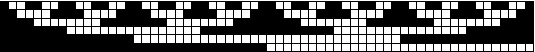
\includegraphics[width=4in]{BRGC6-cropped.pdf} 


\includegraphics[width=4in]{BCLX6-cropped.pdf} 

    \caption{A visual representation of Lexicographic (top), binary reflected Gray code (middle), and cool-lex (bottom) enumerations of 6-bit binary strings. Individual strings are read vertically with the most significant bit at the top; white is 1.
    }
    \label{binary}
\end{figure}

\section{Cool-Lex Order} \label{sec:coolIntro}

Cool-lex order can most easily be introduced using marbles on a ramp. Suppose one has $n$ marbles on a ramp, with each marble colored black or white.  

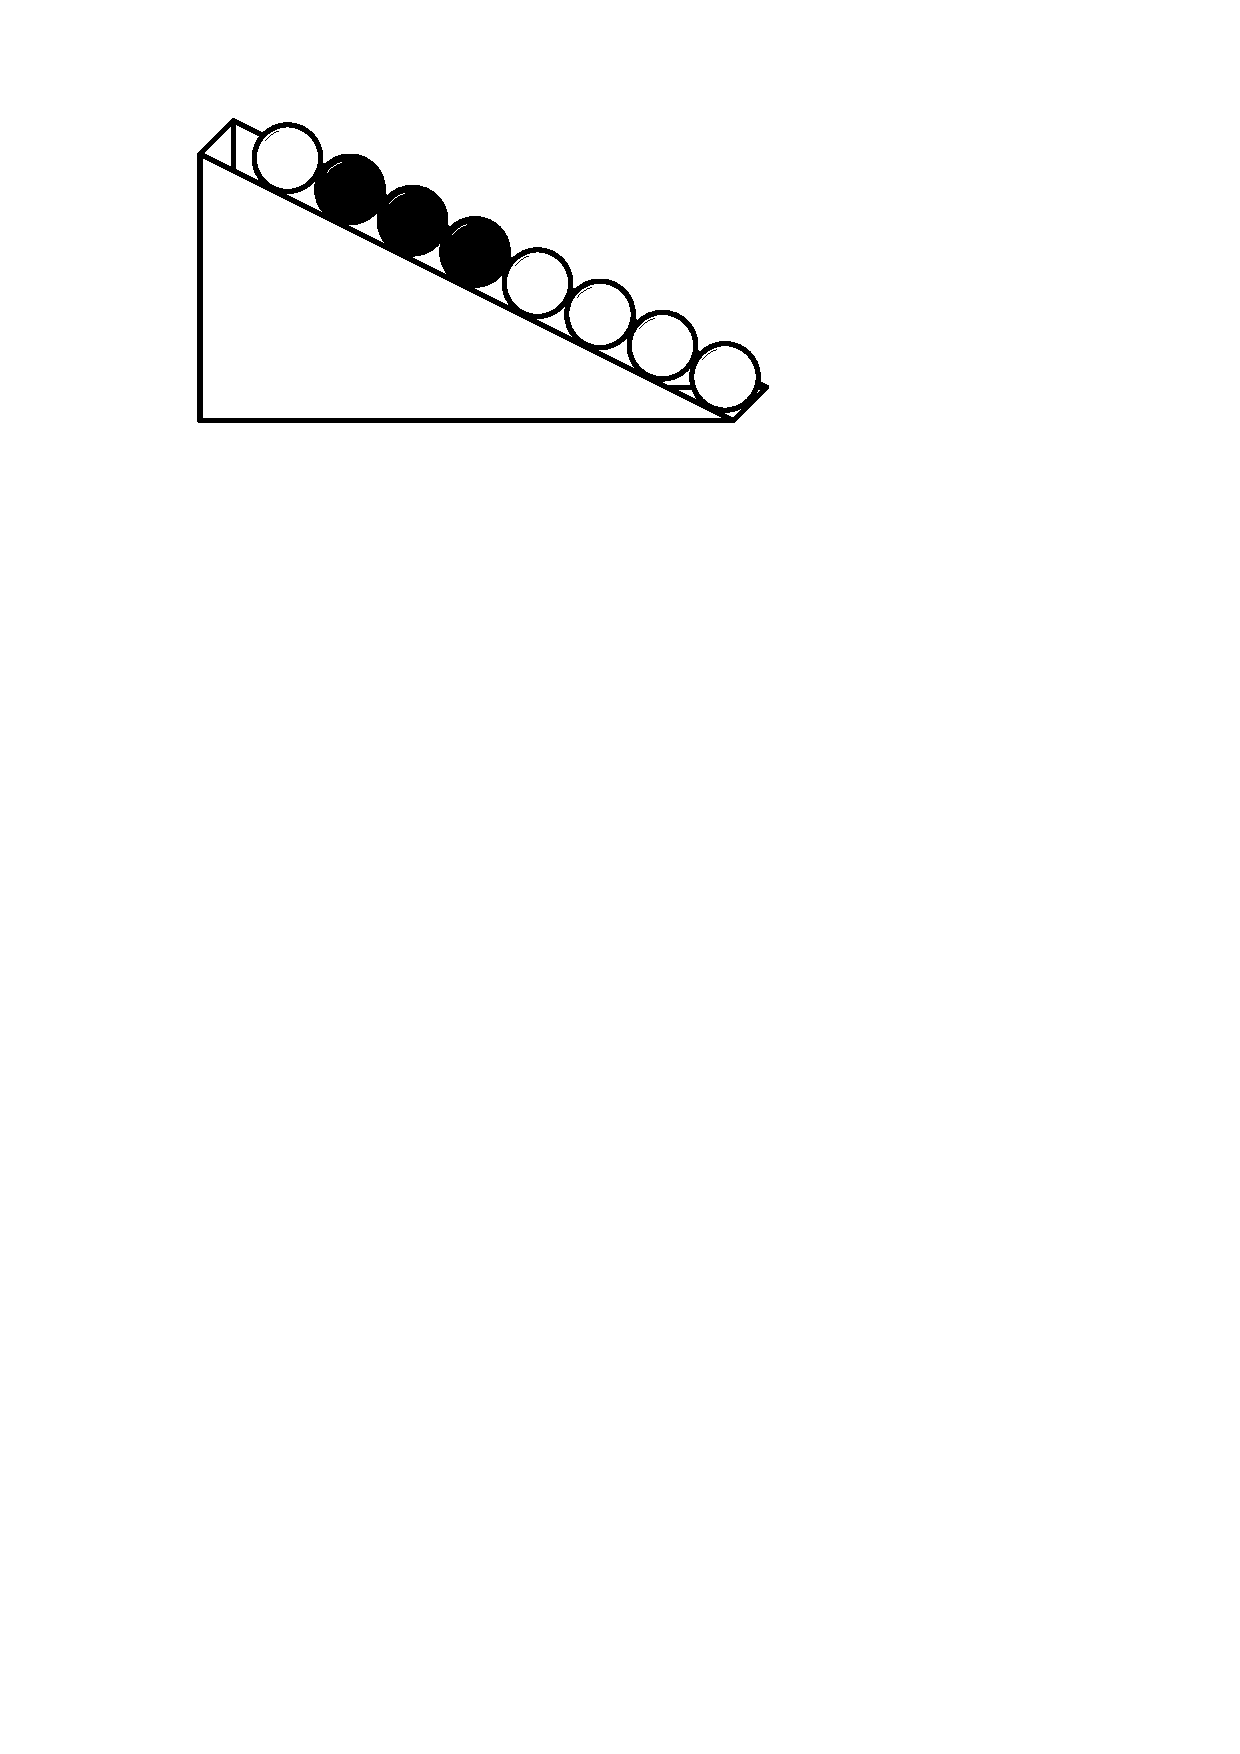
\includegraphics[width=.3\textwidth]{figures/marbles_first.pdf} 


Let $x$ be the first black marble that follows a white marble. Consider picking up and moving marble $x+1$ to the top of the ramp. This yields a new configuration.

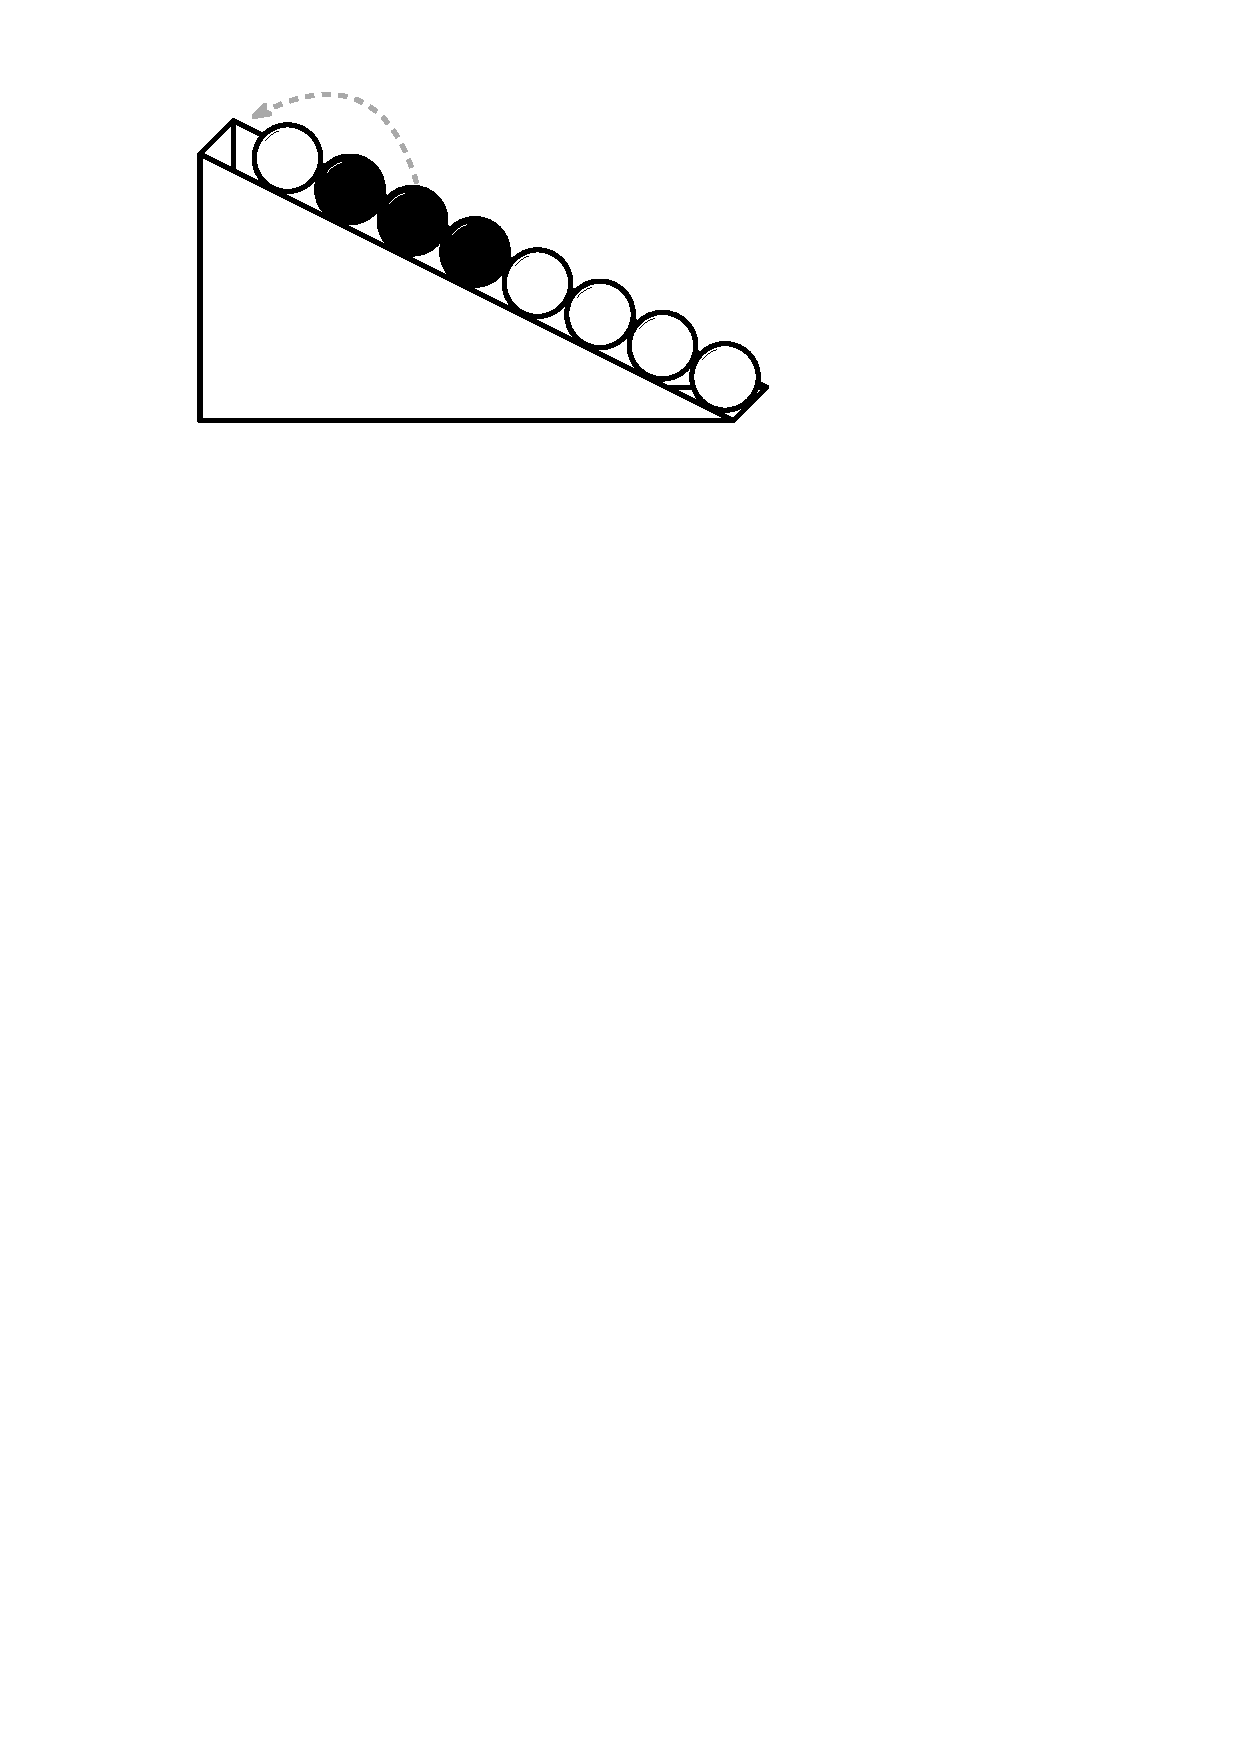
\includegraphics[width=.3\textwidth]{figures/marbles_first_arrow.pdf} $\implies$
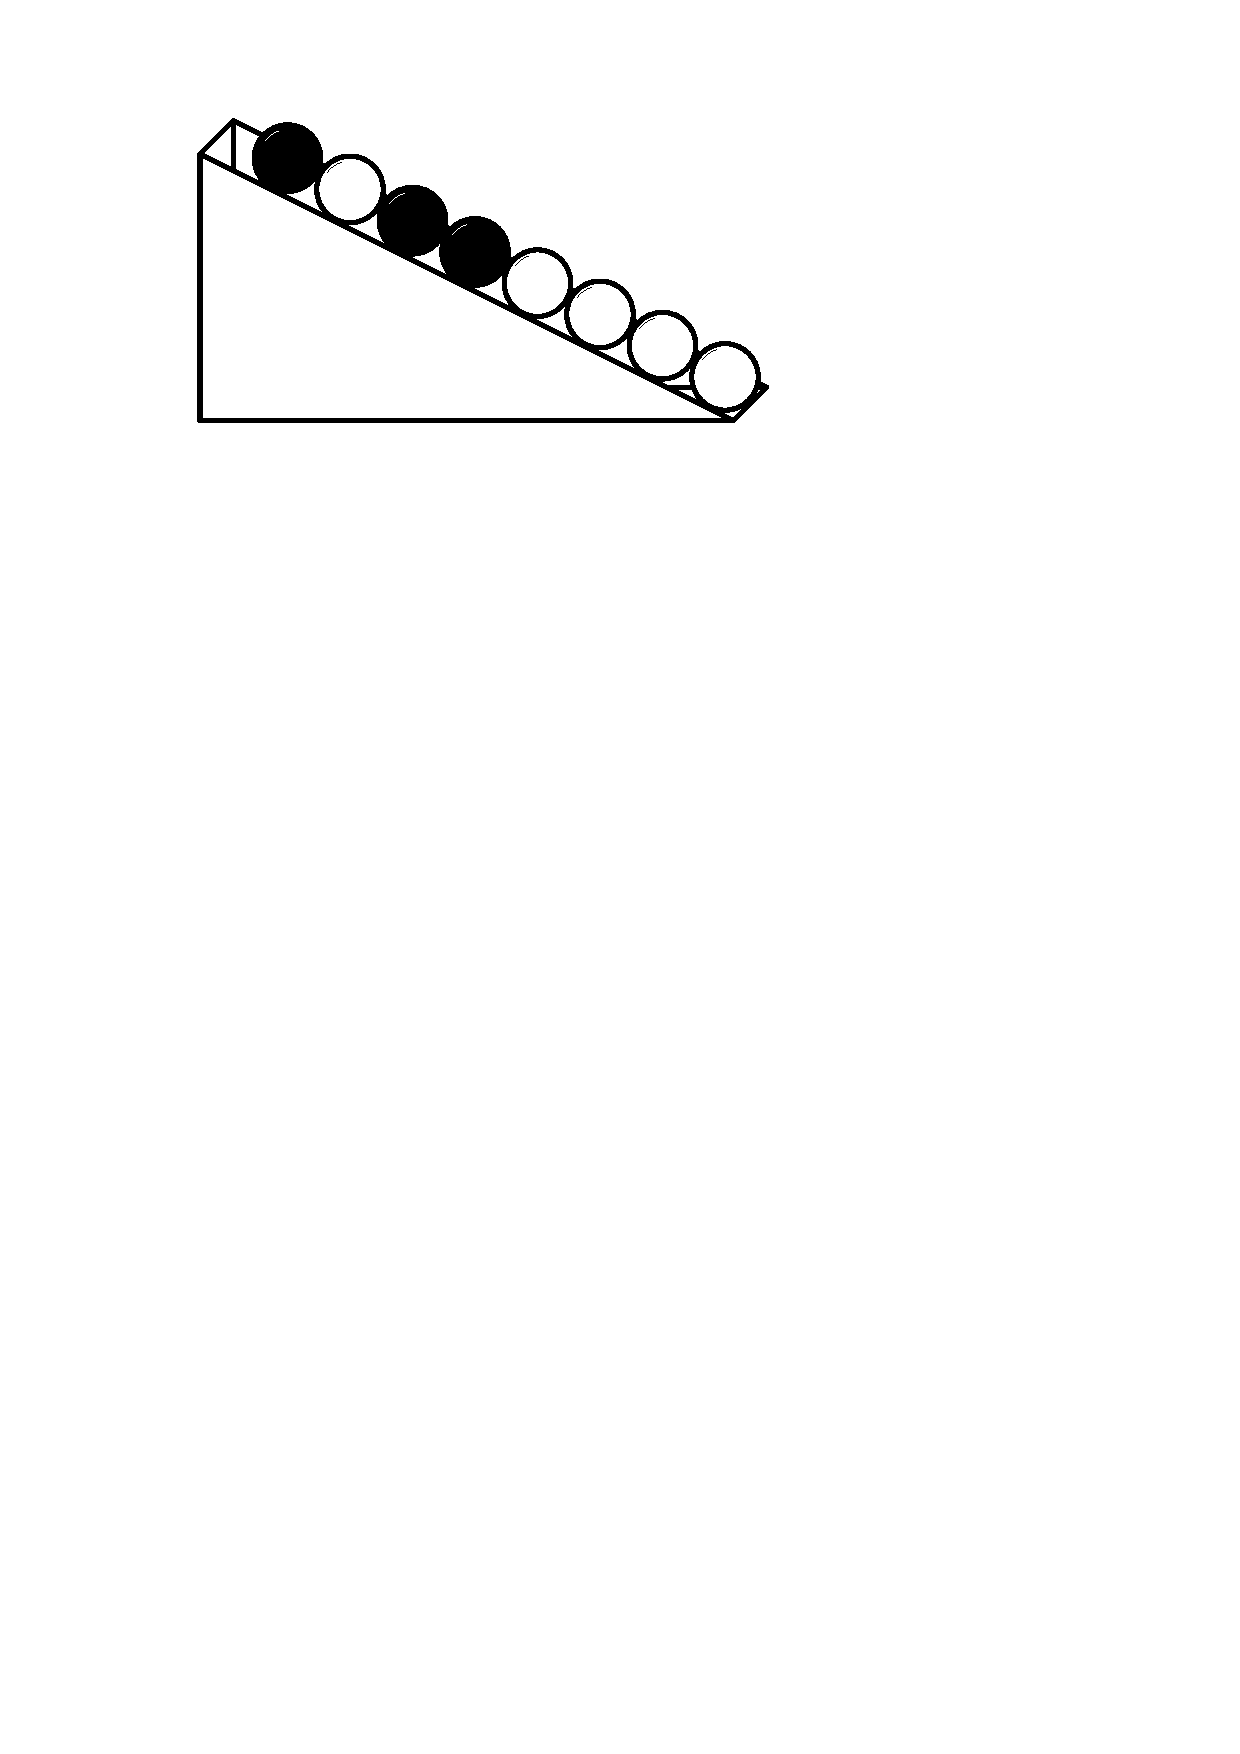
\includegraphics[width=.3\textwidth]{figures/marbles_second.pdf} 

Now, consider performing the same move again: finding $x$, the first black marble that follows a white marble, and moving marble $x+1$ to the top of the ramp. This yields a third configuration.

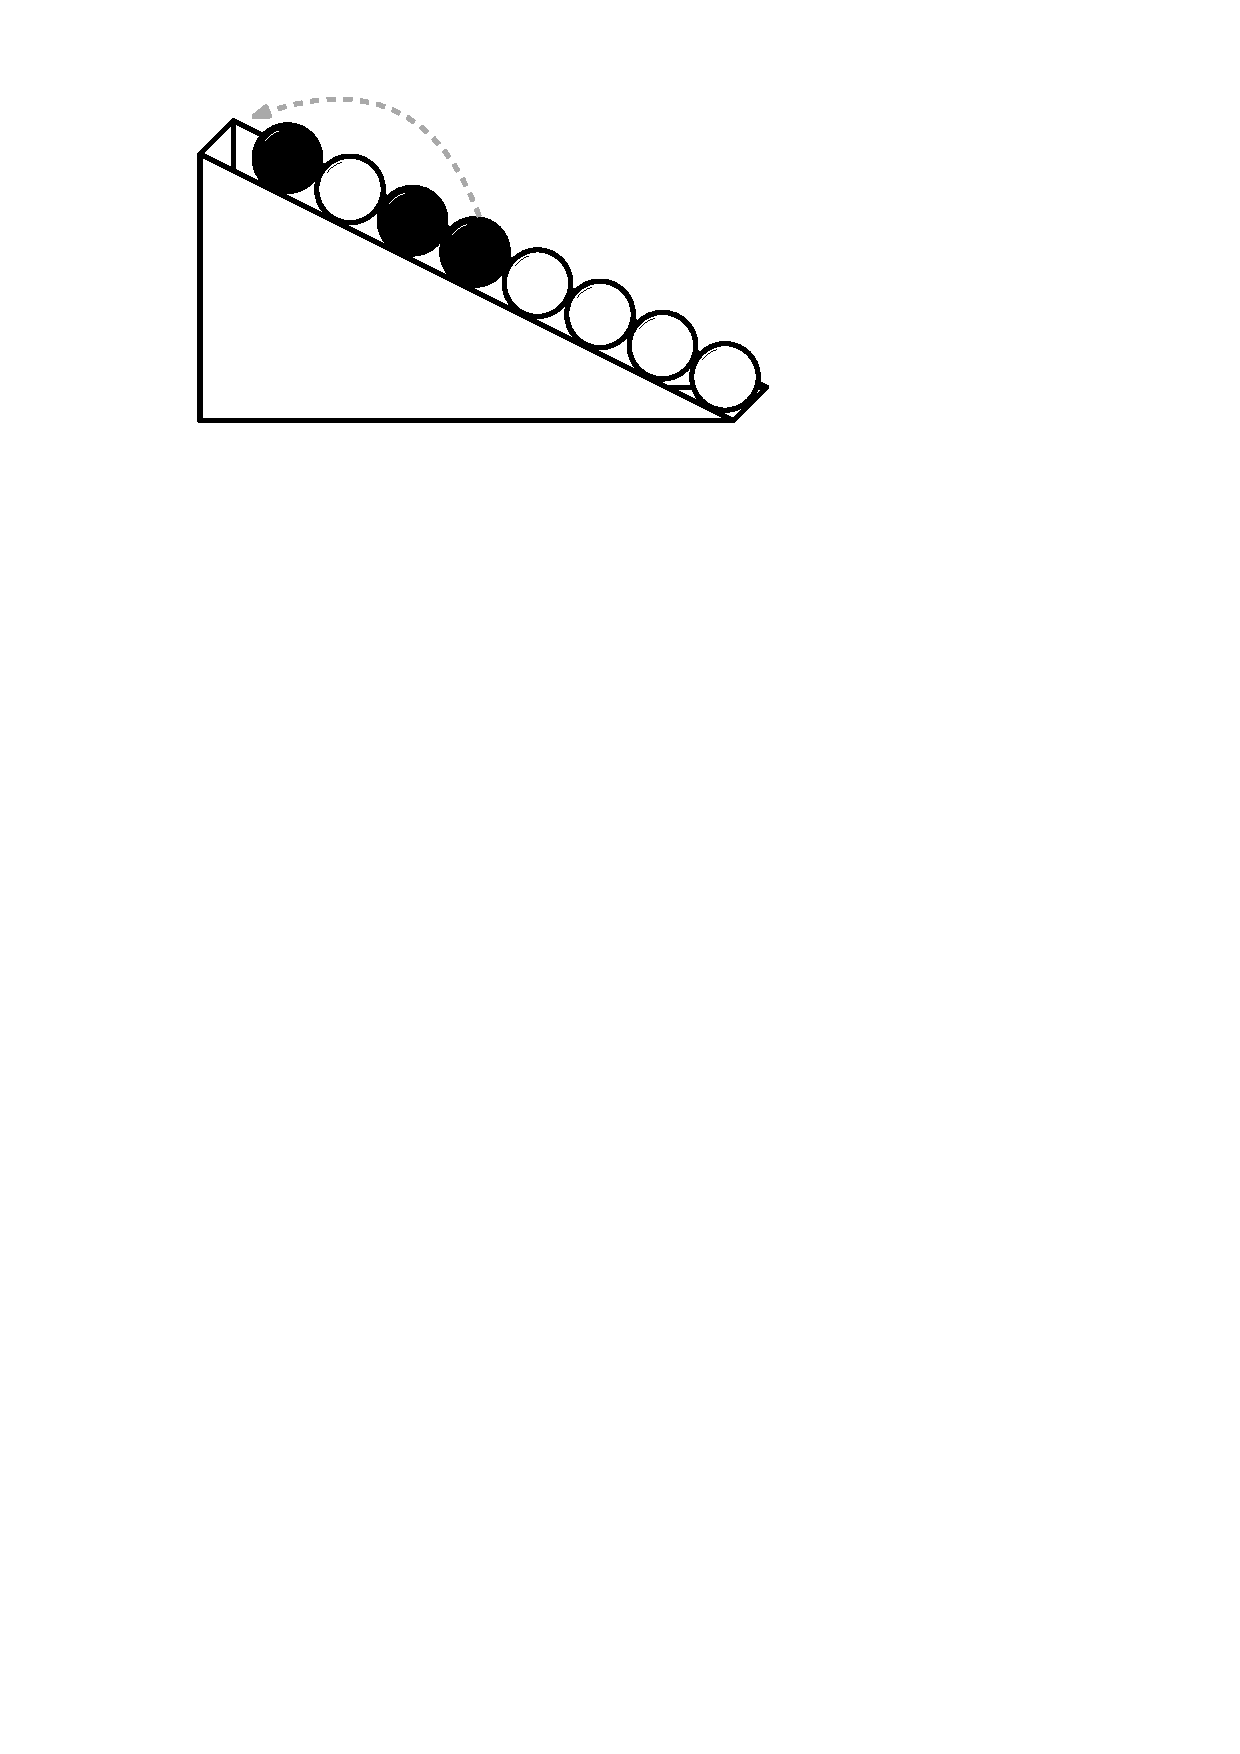
\includegraphics[width=.3\textwidth]{figures/marbles_second_arrow.pdf} $\implies$
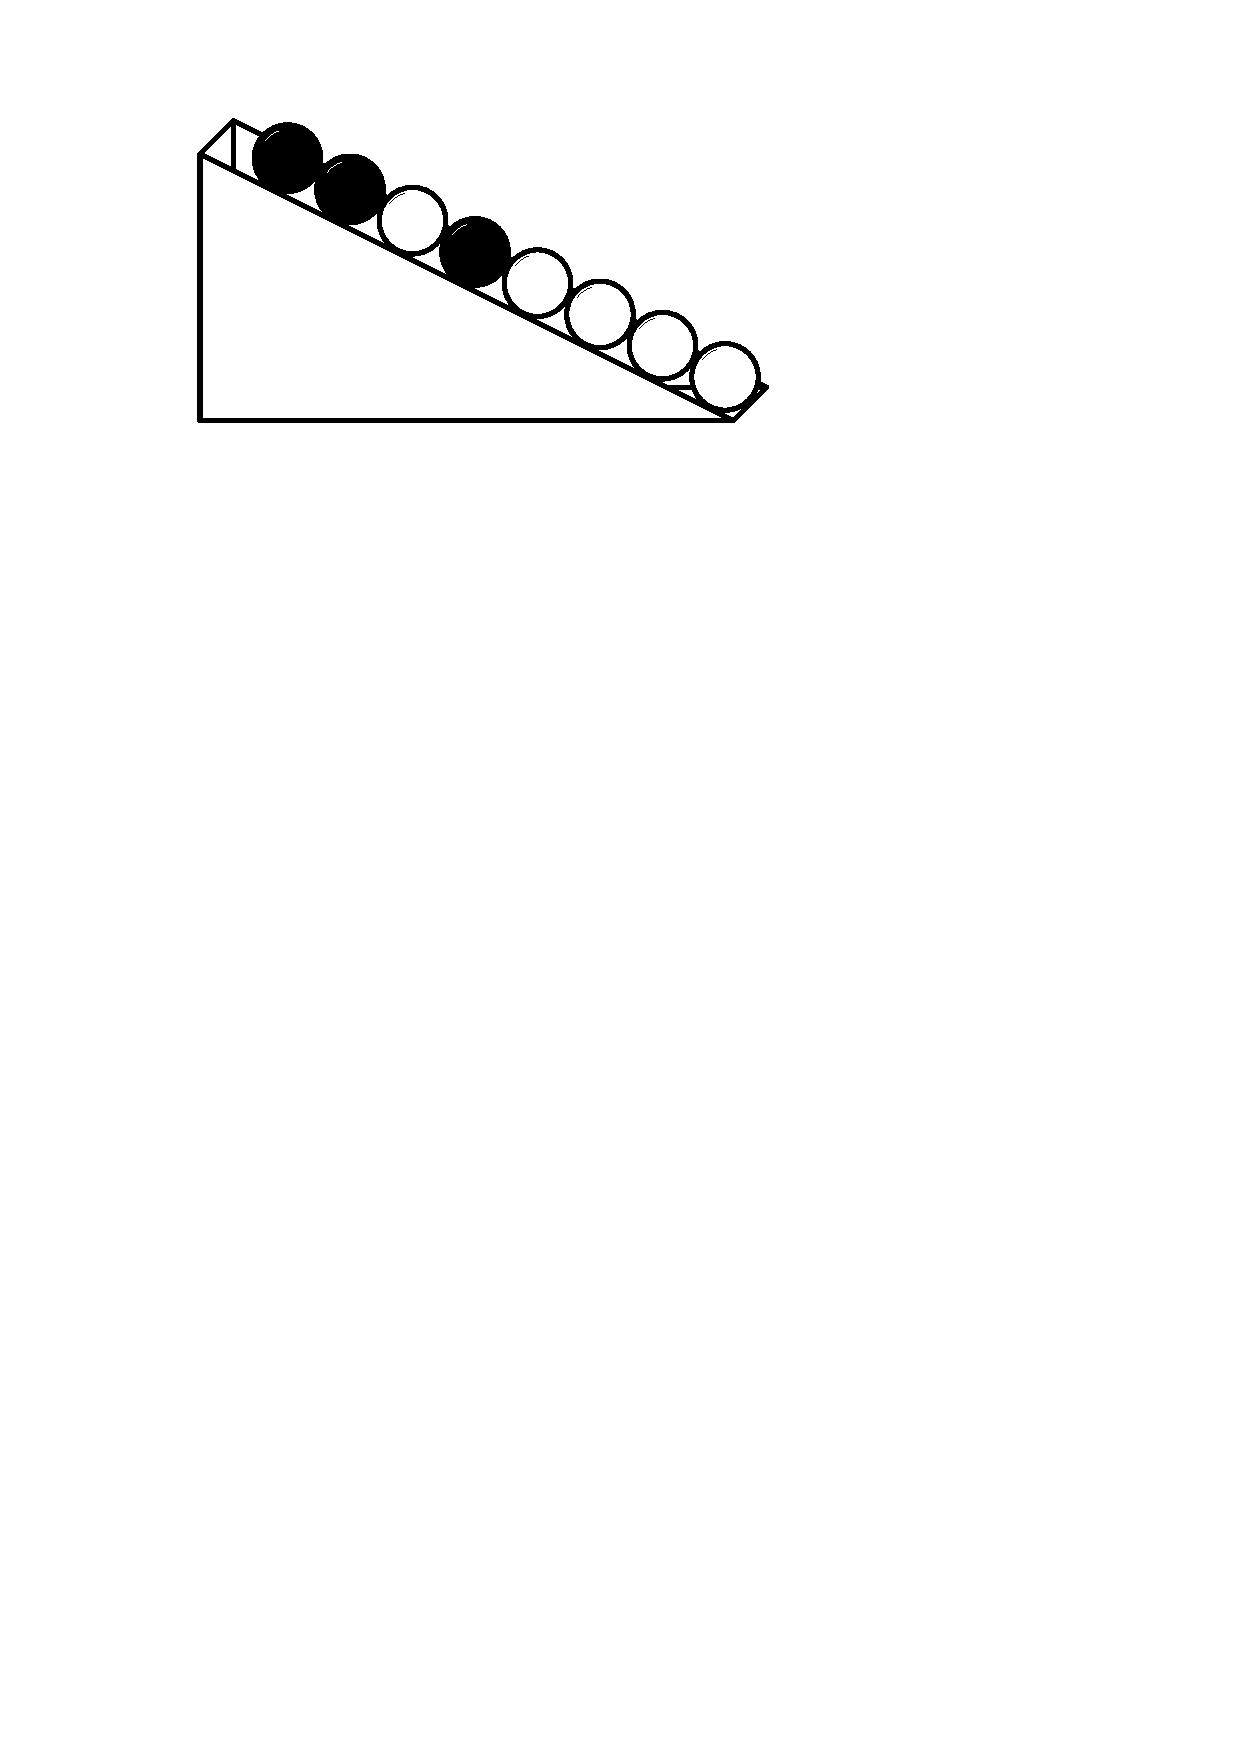
\includegraphics[width=.3\textwidth]{figures/marbles_third.pdf} 

Amazingly, repeatedly performing this operation will eventually generate all possible marble arrangements (with no distinction made between individual black and white marbles). To make the order cyclic, add an additional rule for the case where no black marble follows a white marble (all black marbles come before all white marbles).  In this case, shift the last marble to the top of the ramp.

This rule for marbles on a ramp can be translated to binary strings to create a successor rule that generates all binary strings with fixed content.  We refer to this operation of moving a single marble to the top of the ramp as a \emph{left-shift}.
The order described by this rule is 
cool-lex order, a variation of co-lexicographic order that was first introduced for $(s,t)$-combinations by Ruskey and Williams \cite{ruskey2005generating} \cite{ruskey2008generating}.  It was initially discovered by thinking about simple iterative successor rules like the successor rule for the binary reflected Gray code in equation \ref{eq:BRGC-rule}. To generate all binary strings of a given length instead of all binary strings with a fixed set of content, one only needs to change the rule slightly.  In the case where there is no black marble following a white marble, move the last marble to the top of the ramp and change its color.  In binary strings, this rule corresponds to left-shifting the last bit to the front of the string and complementing it.

Cool-lex order has some advantages of both lexicographic orderings and Gray codes.  Like lexicographic orders, cool-lex order has a simple recursive structure that is easy to understand at  high level.  
Like the binary reflected Gray code, cool-lex orders often lead to generation algorithms that are simpler and more efficient than lexicographic orders.  Accordingly, cool-lex objects for exhaustively generating different sets are not just of theoretical interest.
For example, the ``multicool" package in R uses a loopless cool-lex algorithm to efficiently enumerate multiset permutations.   The package started using cool-lex order for multiset permutations in version 1.1 and as of version 1.12 has been downloaded nearly a million times \cite{multicool_2021}.  Moreover, due to its efficiency and simplicity, Don Knuth included the cool-lex algorithm for combinations in his 4th volume of \emph{The Art of Computer Programming} and provided an implementation of it for his theoretical MMIX processor architecture due to its efficiency and simplicity \cite{knuth2015art}.  Additionally, a hardware implementation of the cool-lex order for combinations in a FPGA was introduced during Madeline Burbage's award winning ACM student research presentation \cite{burbage2020cool}.

% In addition to these, applications of cool-lex order are rapidly growing and new cool-lex algorithms are being discovered every year.  




\subsection{Cool-Lex Sublists}

Like the binary reflected Gray code, cool-lex order has also been used to create additional minimal change orders via taking sublists. In particular, a binary \emph{bubble language} is a set of binary strings with the closure property that the first $01$ of any string can be replaced by $10$ to obtain another string in th set.  Ruskey, Sawada, and Williams found that all binary \emph{bubble languages} appear in a Gray code order when listed in cool-lex order.  Specifically, any binary bubble language can be listed in cool-lex order such that successive strings differ by one or two transpositions.  The approach used in this paper is similar to that discussed in \cite{sawada2021inside} for generating Gray codes for ``flip-swap" languages.  A Gray code can be obtained for any \emph{fixed weight} binary bubble language, or a binary bubble language that is a subset of $(s,t)$-combinations, by generating all $(s,t)$-combinations and filtering to contain strings in the relevant language.  Gray codes for bubble languages of varying weights can be obtained by concatenating fixed weight binary bubble language Gray codes together.
Importantly, although this approach initially involves generating a superset of a language and filtering, careful analysis of the filtered order can typically yield a direct successor rule that efficiently generates only strings in the language without filtering.  This has allowd for different versions of cool-lex order to efficiently enumerate Dyck words and binary trees \cite{ruskey2008generating}, k-ary Dyck words, \cite{durocher2012cool}, and fixed-density necklaces and other languages \cite{sawada2009fixed}.  

In addition to the cool-lex order for $(s,t)$-combinations and bubble languages, cool-lex order has been generalized to enumerate other languages as well.  In particular, cool-lex order for all binary strings of a given length \cite{stevens2012coolest} and multiset permutations \cite{williams2009loopless} have been developed as well.  Our result in Chapter \ref{chap:luka-graycode} will provide a Gray code for a subset of multiset permutations in cool-lex order that was obtained initially by filtering the cool-lex order for multiset permutations.  The resulting rule generates fixed-content Lukasiewicz words using one left-shift per generated string.


\section{Gray Codes for Trees and Catalan Objects} \label{sec:intro_Graycodes}

This thesis aims to create efficient minimal change orderings for other objects, namely ordered trees and Lukasiewicz words.  Ordered trees and Lukasiewicz words are both \emph{Catalan objects}.  The number of Lukasiewicz words of length $n+1$ and the number of ordered trees with $n+1$ nodes are both counted by the $n\thh$ Catalan number $\C_n$.  

Frank Gray's reflected binary code used complementing a single bit as the minimal change between successive binary strings in its ordering.  Other notions of minimal changes in strings are \emph{adjacent-transpositions}, or \emph{swaps}, which interchange two adjacent symbols in a string, and \emph{shifts}, in which a single symbol in a string moved to another position. Lukasiewicz words are typically represented as strings of integers, and therefore can make use of these minimal change string operations.  Our Gray codes for Lukasiewicz words will use a slightly more restrictive type of shift, a \emph{left-shift}, which moves a single symbol somewhere to the left within a string. 



% PICTURE? ESA IMAGE? BUT WITHOUT STACK?

Defining minimal changes for trees is more complicated, as what changes are \emph{minimal} within a tree is often representation dependent.  Our Gray code for ordered trees aims to use simple operations that are minimal for most reasonable tree representations.  These minimal changes use ``pops", which remove a node's first child, and ``pushes,'' which push one node to be the first child of another.  More specifically, the algorithm will generate trees using a pop-push operation that pops one node's first child and pushes it to become the first child of another node.  We will refer to this pop-push operation as a ``pull.''

% TODO: picture



\section{Goals and Results}


This thesis has the broad goal of extending cool-lex order to new objects.  It provides two primary contributions, each with sub-contributions.  

The first contribution is a `pop-push' Gray code for enumerating ordered trees in $O(1)$ time. Chapter \ref{chap:otree-graycode} will give a two-case successor rule for generating all ordered trees with $n$ nodes using at most two ``pull'' operations. Chapter \ref{chap:otree-implementation} will provide a loopless algorithm for the successor rule in \ref{chap:otree-graycode} and an implementation of the algorithm in C.  This algorithm is an extension of the cool-lex order for Dyck words and binary trees presented by Ruskey and Williams. It shows that the cool-lex order for Dyck words is simultaneously a Gray code for a third Catalan object: ordered trees, as well as Dyck words and binary trees.  These results have been submitted to an international algorithms conference and are currently under review \cite{lapeypush}.

The second contribution is a shift Gray code for Lukasiewicz words.  Lukasiewicz words are a generalization of Dyck words that allow for broader sets of content while maintining a notion of ``balance." Chapter \ref{chap:luka-graycode} will give a shift Gray code for generating Lukasiewicz words with fixed content using one prefix shift per iteration.  Chapter \ref{chap:luka-implementation} will give a loopless implementation of the algorithm in \ref{chap:luka-graycode} using an array based implementation for the special case of Motzkin words and a linked list implementation for the general case of unrestricted Lukasiewicz words.  These results have been accepted at the 33rd International Workshop on Combinatorial Algorithms and will be presented June 2022 \footnote{Although these results are presented after the ordered trees result in this paper, these results were developed earlier and therefore were submitted to an earlier conference} \cite{lapey2022shift}.

Chapter \ref{chap:catalan} will give background information on the Catalan numbers and their relation to the combinatorial objects generated by this thesis.  Chapter \ref{chap:cool} will give background information on existing applications of cool-lex order.  Chapters \ref{chap:otree-graycode} and \ref{chap:otree-implementation} will give a new successor rule and loopless implementation for generating ordered trees in cool-lex order.  Chapter \ref{chap:luka-background} will give background information on generalizations of Dyck words, including Lukasiewicz words and Motzkin words. Chapters \ref{chap:luka-graycode} and \ref{chap:luka-implementation} will give a successor rule and loopless implementation for generating fixed-content Lukasiewicz words.
